\documentclass[12pt,a4paper,oneside]{report}

\usepackage[margin=1in]{geometry}
\usepackage[T1]{fontenc}
\usepackage[utf8]{inputenc}
\usepackage{lmodern}
\usepackage{microtype}
\usepackage{booktabs}
\usepackage{array}
\usepackage{longtable}
\usepackage{enumitem}
\usepackage{xcolor}
\usepackage{hyperref}
\usepackage{listings}
\usepackage{amsmath}
\usepackage{amssymb}
\usepackage{graphicx}
\usepackage{float}

\hypersetup{
  colorlinks=true,
  linkcolor=blue!45!black,
  citecolor=blue!45!black,
  urlcolor=blue!45!black,
  pdftitle={Accelera Auto Preprocessing, Reporting, and Benchmarking Modules},
  pdfauthor={Individual Work Draft}
}

\lstdefinestyle{pythonstyle}{
  language=Python,
  basicstyle=\ttfamily\small,
  keywordstyle=\color{blue!60!black},
  commentstyle=\color{green!40!black},
  stringstyle=\color{red!55!black},
  frame=single,
  breaklines=true,
  columns=fullflexible,
  keepspaces=true,
  showstringspaces=false
}

\lstdefinestyle{algostyle}{
  basicstyle=\ttfamily\small,
  frame=single,
  breaklines=true,
  columns=fullflexible,
  keepspaces=true,
  showstringspaces=false
}

\newcommand{\systemname}{Accelera}
\newcommand{\modulepath}[1]{\texttt{\detokenize{#1}}}
\newcommand{\todoitem}[1]{\textcolor{red!65!black}{[TODO: #1]}}

\title{
  \vspace{-1.5cm}
  \textbf{Accelera Auto Preprocessing, Reporting, and Benchmarking Modules}\\[0.4em]
  \Large Data Preparation, Automated Reports,\\
  and Fair Benchmark Evaluation
}
\author{
  Individual Work\\[0.5em]
  Nesma Osama\\
  ID: 9220912\\[0.6em]
  Supervisor: Dr. Salma Abdel Monem
}
\date{June 2026}

\begin{document}

\maketitle

\begin{abstract}
This report describes three separate parts of the \systemname{} project:
the Auto Preprocessing module, the Reporting module, and the Benchmarking
module. The Auto Preprocessing module prepares tabular, text, and image
datasets by applying rule-based cleaning, transformation, artifact saving, and
optional exploratory reports. The Reporting module focuses on the report
generation code that exists inside the \modulepath{accelera_pipe} package and the preprocessing
wrappers. It is treated here as a reporting component, not as a full discussion
of workflow construction. The Benchmarking module provides a web-based
environment where users can create benchmark tasks, submit prediction files,
and compare results using selected evaluation metrics.

The contribution of this draft is the design and implementation documentation
of these modules, not a claim that they outperform existing systems. The
present chapters describe the problem, background concepts, methodology,
source-code organization, report generation behavior, benchmarking workflow,
testing, and current limitations. Each implementation claim is tied to a class,
file, or data flow that exists in the repository.
\end{abstract}

\tableofcontents
\listoftables
\clearpage

% -----------------------------------------------------------------------------
\chapter{Introduction}
\label{chap:introduction}

\section{Background}

In many machine-learning projects, the model is not the only important part.
Before training a model, the dataset usually needs to be cleaned, explored,
split, encoded, scaled, and checked for errors. The user also needs reports
that explain what happened during preprocessing or evaluation. If different
users are trying different solutions, there must also be a fair way to compare
their predictions.

\systemname{} tries to support these steps as one framework. The Auto
Preprocessing module handles repeated data preparation work. The Reporting
module produces HTML reports and graphs that make the output easier to
understand. The Benchmarking module adds a higher-level evaluation workflow
where a benchmark creator defines the task and other users submit predictions.

\section{Problem Statement}

The problem addressed in this work can be written as:

\begin{quote}
How can \systemname{} reduce repetitive preprocessing work, generate readable
reports, and provide a fair benchmark workflow for comparing machine-learning
submissions?
\end{quote}

This problem contains three smaller problems:

\begin{enumerate}[leftmargin=*]
  \item automatically preparing tabular, text, and image datasets for training
        and testing;
  \item generating reports that make preprocessing output and evaluation
        results understandable to the user; and
  \item evaluating prediction submissions using the same target file and metric
        rules for all users.
\end{enumerate}

\section{Motivation}

Manual preprocessing is repetitive and can easily become inconsistent between
training and testing. For example, if one encoder is fitted on the training
data but a different encoder is used on the test data, the model may receive
wrong feature values. The same issue happens when columns are dropped manually
without saving the decision. Therefore, the preprocessing module saves fitted
objects and metadata so the same transformations can be applied later.

Reporting is also important because preprocessing and evaluation can produce
many details. A user needs to know what columns were dropped, what graphs were
generated, what features were selected, and what metric results were produced.
The report code solves this by collecting structured report data and converting
it into HTML pages, images, tables, and metric summaries.

Finally, benchmarking requires a clear separation between the test features and
the ground-truth target. The Benchmarking module uses this separation so all
submissions are scored under the same rules.

\section{Scope}

This report focuses on the implemented material available in the repository:

\begin{itemize}[leftmargin=*]
  \item Auto Preprocessing for tabular, text, and image data;
  \item Reporting code used by preprocessing and graph report outputs;
  \item Benchmarking module backend, frontend, validation, and scoring design; and
  \item testing and comparison notes already documented in the project report.
\end{itemize}

The report does not describe AutoML search in detail because that is covered in
a separate individual-work file. It also does not claim a complete production
benchmarking service, because some parts are still described as project-level
functionality.

\section{Objectives}

The objectives of this work are:

\begin{itemize}[leftmargin=*]
  \item automate common preprocessing decisions based on dataset type;
  \item avoid training-test preprocessing mismatch by saving artifacts;
  \item generate understandable reports for preprocessing and metric results;
  \item separate report generation from the main preprocessing and benchmarking
        workflows;
  \item use metrics in a general way through scikit-learn metric functions;
  \item provide a benchmark workflow for benchmark creation, submission, and
        leaderboard display; and
  \item document the source-code structure in a way that can be reviewed and
        extended later.
\end{itemize}

% -----------------------------------------------------------------------------
\chapter{Background and Related Concepts}
\label{chap:background}

\section{Data Preprocessing}

Data preprocessing is the stage where raw data is converted into a clean and
usable format. This can include missing value handling, duplicate removal,
encoding categorical values, scaling numerical values, feature selection, and
splitting data into training and validation sets. In this project,
preprocessing is treated as a reusable workflow, not as a one-time notebook
step.

\section{Exploratory Data Analysis}

Exploratory Data Analysis, or EDA, helps the user understand the dataset before
model training. It includes statistics such as missing values, duplicate
counts, column types, unique values, and distributions. The preprocessing report
uses these values so the user can see what existed before and after processing.

\section{Tabular, Text, and Image Data}

Different data types need different preprocessing logic. Tabular data is stored
as rows and columns, so the system detects numerical, categorical, binary,
ordinal, and unsupported columns. Text data must be cleaned and transformed
into numerical vectors, so TF-IDF is used. Image data is represented by image
files in class folders, so the system validates images, maps classes to labels,
resizes images, and creates data loaders.

\section{Automated Reporting}

Automated reporting means collecting important information during execution and
turning it into a readable output for the user. In this work, reports are used
for two main purposes. First, preprocessing reports explain the original data,
the applied preprocessing steps, and the final transformed output. Second,
metric and graph reports explain evaluation results using tables, figures, and
HTML sections.

\section{Benchmarking}

Benchmarking is the process of comparing different solutions on the same task.
In this project, a benchmark has a dataset, a test dataset, a ground-truth
target file, a problem type, and an evaluation metric. A submission is a
prediction file plus a repository link. The Benchmarking module scores each
submission and displays the result in a leaderboard.

\chapter{Auto Preprocessing Methodology}
\label{chap:auto-preprocessing}

\section{Module Overview}

The Auto Preprocessing module is implemented under
\modulepath{accelera/src/auto_preprocessing}. It contains a core package for
training and testing preprocessing classes, and a wrappers package for report
graphs and HTML report generation.

The module supports three dataset families:

\begin{itemize}[leftmargin=*]
  \item tabular datasets for classification and regression;
  \item text datasets for classification; and
  \item image datasets for classification.
\end{itemize}

The workflow starts from the raw data and user configuration. The module then
applies suitable preprocessing steps and saves both the processed output and
the fitted objects required for later use.

\section{Source-Code Organization}

\begin{table}[H]
\centering
\caption{Auto Preprocessing implementation units}
\label{tab:auto-preprocessing-units}
\begin{tabular}{p{0.48\textwidth}p{0.52\textwidth}}
\toprule
File or directory & Responsibility \\
\midrule
\modulepath{core/preprocessing_base.py} & Common base interface for
preprocessing classes. \\
\modulepath{core/training_tabular_preprocessing_base.py} & Shared tabular
training behavior such as data overview, duplicate removal, and splitting. \\
\modulepath{core/classical_training_preprocessing.py} & Main tabular
training preprocessing implementation. \\
\modulepath{core/classical_testing_preprocessing.py} & Test-time tabular
preprocessing using saved training artifacts. \\
\modulepath{core/text_training_preprocessing.py} & Text cleaning,
tokenization, TF-IDF transformation, target encoding, and reporting. \\
\modulepath{core/text_testing_preprocesing.py} & Text test-time
preprocessing using saved vectorizer and label encoder. \\
\modulepath{core/classification_image_training_preprocessing.py} & Image
classification data validation, class mapping, splitting, loading, and report
generation. \\
\modulepath{core/classification_image_testing_preprocessing.py} & Image
test-time preprocessing using saved image size and class mapping. \\
\modulepath{wrappers/tabular_preprocessing_report.py} & HTML report for
tabular and text preprocessing. \\
\modulepath{wrappers/image_preprocessing_report.py} & HTML report for image
preprocessing. \\
\bottomrule
\end{tabular}
\end{table}

\section{Tabular Training Flow}

The tabular training flow is implemented mainly in
\modulepath{classical_training_preprocessing.py}. The class receives a pandas
DataFrame, target column, problem type, folder path, validation size, random
state, thresholds, and report flag.

The training flow is:

\begin{enumerate}[leftmargin=*]
  \item validate the input configuration;
  \item save original data columns for later testing;
  \item create a data overview for the report;
  \item remove duplicate rows;
  \item split data into training and validation sets;
  \item detect columns that should be dropped;
  \item detect each column type;
  \item generate graphs if reports are enabled;
  \item build a column transformer for feature preprocessing;
  \item preprocess the target according to classification or regression;
  \item apply feature selection using mutual information;
  \item save all fitted objects and metadata; and
  \item generate the HTML report.
\end{enumerate}

\begin{lstlisting}[style=algostyle,caption={General tabular preprocessing flow}]
Input: DataFrame D, target column y, problem type
Output: X_train, X_val, y_train, y_val

1:  Validate configuration
2:  Store original dataset columns
3:  Build data overview and report information
4:  Remove duplicate rows
5:  Split into training and validation sets
6:  Drop user-selected, high-missing, constant, and unsupported columns
7:  Detect column types from training data
8:  Generate feature and target graphs when report is enabled
9:  Fit feature preprocessing objects on X_train
10: Transform X_train and X_val
11: Fit target preprocessing object on y_train
12: Transform y_train and y_val
13: Select useful features using mutual information
14: Save fitted objects and metadata
15: Generate report if enabled
\end{lstlisting}

\section{Tabular Column Type Detection}

The module assigns a type to each feature and then chooses preprocessing based
on the type. This rule-based design is easy to understand and works without
writing special code for every dataset.

\begin{table}[H]
\centering
\caption{Detected tabular column types and preprocessing}
\label{tab:column-types}
\begin{tabular}{p{0.30\textwidth}p{0.60\textwidth}}
\toprule
Column type & Applied preprocessing \\
\midrule
Numerical and continuous & Median imputation followed by robust scaling. \\
Binary & Most-frequent imputation followed by ordinal encoding. \\
Ordinal & Most-frequent imputation followed by robust scaling. \\
Low-cardinality categorical & Most-frequent imputation followed by binary
encoding. \\
High-cardinality categorical & Most-frequent imputation followed by frequency
encoding. \\
Unsupported or other & Removed from the preprocessing pipeline. \\
\bottomrule
\end{tabular}
\end{table}

\section{Target Processing}

For classification, the target is encoded using a label encoder. Missing target
values are filled using the most frequent target class. For regression, the
target is scaled using a robust scaler. The fitted target preprocessor is saved
as \modulepath{target_preprocessor.pkl}, so predictions or test labels can be
converted consistently later.

\section{Feature Selection}

After feature preprocessing, the module applies mutual-information based
feature selection. For classification it uses mutual information for
classification tasks, and for regression it uses mutual information for
regression tasks. The selected features are saved in
\modulepath{selected_features.pkl}. This reduces unnecessary feature columns
and keeps the testing stage aligned with training.

\section{Saved Tabular Artifacts}

\begin{table}[H]
\centering
\caption{Saved artifacts for tabular preprocessing}
\label{tab:tabular-artifacts}
\begin{tabular}{p{0.36\textwidth}p{0.54\textwidth}}
\toprule
Artifact & Purpose \\
\midrule
\modulepath{data_columns.pkl} & Original input columns before preprocessing. \\
\modulepath{col_drop.pkl} & Columns removed during training preprocessing. \\
\modulepath{training_preprocessor.pkl} & Fitted feature transformer. \\
\modulepath{feature_names.pkl} & Names of generated transformed features. \\
\modulepath{target_preprocessor.pkl} & Fitted label encoder or target scaler. \\
\modulepath{target_info.pkl} & Target metadata used during testing. \\
\modulepath{bool_type_col.pkl} & Boolean columns that need consistent handling. \\
\modulepath{selected_features.pkl} & Feature indices or names selected after
mutual information. \\
\bottomrule
\end{tabular}
\end{table}

\section{Tabular Testing Flow}

The testing class loads the saved artifacts and applies the same
transformations to new data. This is important because the testing data must
not fit a new preprocessor. It should only use what was fitted during training.
The test data is checked against the saved column list, dropped columns are
removed, feature preprocessing is applied, selected features are kept, and the
target is transformed if it exists.

\section{Text Training Flow}

The text preprocessing class is used when the dataset contains a text column
and a target column. It inherits shared tabular behavior for overview,
duplicates, and splitting, but it uses text-specific feature preprocessing.

The text flow is:

\begin{enumerate}[leftmargin=*]
  \item generate a dataset overview;
  \item remove duplicate rows;
  \item split into training and validation sets;
  \item generate optional graphs such as target distribution and top word
        frequency;
  \item fill missing text values with an empty string;
  \item clean and tokenize text;
  \item transform text using TF-IDF;
  \item encode the target labels;
  \item save TF-IDF vectorizer, label encoder, and metadata; and
  \item generate the report if enabled.
\end{enumerate}

\section{Text Tokenization}

The custom tokenizer lowercases the text, handles common contractions, keeps
important negation words such as \texttt{not} and \texttt{no}, removes noise
characters, removes short tokens, and applies stemming. This makes the text
more regular before TF-IDF vectorization.

\section{Image Training Flow}

The image classification preprocessing class expects a folder structure where
each class has its own folder. It scans the folders, builds class-to-label and
label-to-class mappings, validates images, optionally splits the training
folder into training and validation sets, applies resizing and augmentation,
and returns PyTorch data loaders.

The image path saves:

\begin{itemize}[leftmargin=*]
  \item class-to-label mapping;
  \item label-to-class mapping;
  \item image size information; and
  \item report data about valid and invalid images.
\end{itemize}

\section{Preprocessing Reports}

The preprocessing report classes reuse the same basic HTML report base from the
reporting code. For tabular and text preprocessing, the report includes the
data overview, duplicate analysis, split information, dropped columns,
preprocessing decisions, generated graphs, feature selection, and processed
data previews. For images, the report includes class distribution, valid and
invalid image counts, split information, and sample visualizations.

This report is useful because preprocessing is usually a hidden part of a
machine-learning project. Here the user can see what the module did instead of
only receiving transformed arrays.

% -----------------------------------------------------------------------------
\chapter{Reporting Module}
\label{chap:reporting}

\section{Module Overview}

The Reporting module is not a completely separate package in the source tree,
but it is a separate responsibility in the project. Its classes are mainly
found in two places. The shared report base and metric display report classes
are under \modulepath{accelera/src/accelera_pipe}, while the preprocessing
report classes and graph wrappers are under
\modulepath{accelera/src/auto_preprocessing/wrappers}.

\begin{table}[H]
\centering
\caption{Reporting implementation units}
\label{tab:reporting-units}
\begin{tabular}{p{0.48\textwidth}p{0.52\textwidth}}
\toprule
File or directory & Responsibility \\
\midrule
\modulepath{accelera_pipe/core/report_base.py} & Defines the common HTML
template, styles, graph display helper, and file writing method. \\
\modulepath{accelera_pipe/core/metric_display.py} & Defines the base class for
metric result display wrappers. \\
\modulepath{accelera_pipe/wrappers/graph_pipeline_report.py} & Groups metric
results and selects the suitable display wrapper based on result type. \\
\modulepath{accelera_pipe/wrappers/graph_report.py} & Builds an HTML report
from a serialized graph file and metric results. \\
\modulepath{accelera_pipe/wrappers/display_*} & Contains display classes for
numbers, arrays, dictionaries, strings, tuples, and plotted figures. \\
\modulepath{auto_preprocessing/wrappers/tabular_preprocessing_report.py} &
Builds the tabular and text preprocessing HTML report. \\
\modulepath{auto_preprocessing/wrappers/image_preprocessing_report.py} &
Builds the image preprocessing HTML report. \\
\modulepath{auto_preprocessing/wrappers/*classification.py} and
\modulepath{*regression.py} & Generate graphs for feature and target
distributions. \\
\bottomrule
\end{tabular}
\end{table}

\section{Report Base Design}

\modulepath{ReportBase} defines shared HTML report behavior. It stores the
start and end HTML content, common styling, graph display helpers, and the
\modulepath{create_html_file} method that writes \modulepath{report.html}.
This class is important because different report classes can reuse the same
structure instead of each one writing a full HTML page from the beginning.

The base report also has a helper for showing saved graph images. It receives a
folder path and image names, checks whether the graph files exist, and adds the
images to the HTML content. This is used by preprocessing reports because most
of their visual results are saved as image files first.

\section{Auto Preprocessing Reports}

The tabular preprocessing report is built by
\modulepath{TabularPreprocessingReport}. It receives a \modulepath{report_data}
dictionary collected during preprocessing. This dictionary contains data
overview, duplicate information, split information, dropped columns, generated
graphs, preprocessing steps, processed previews, feature selection results, and
target-null handling.

The report is created in ordered sections:

\begin{enumerate}[leftmargin=*]
  \item show the original and lowercased data heads;
  \item show dataframe information and statistics;
  \item show missing values, duplicates, and shape;
  \item show duplicate removal results;
  \item show training and validation split information;
  \item show dropped columns and previews after dropping;
  \item show generated graphs;
  \item show each preprocessing decision;
  \item show processed training and validation samples; and
  \item show feature-selection results when they exist.
\end{enumerate}

The image preprocessing report is built by
\modulepath{ImagePreprocessingReport}. It shows training-folder and
validation-folder overview information, class names, number of valid images,
invalid image counts, invalid image paths, data split details, random
validation samples, and graph images generated from the image preprocessing
steps.

\section{Generated Graph Types}

The preprocessing wrappers generate graphs according to the feature type and
task type. For tabular classification, categorical wrappers show category
counts and category-target relationships. For regression, they show
category-target distribution plots. Numerical wrappers show histograms,
null-vs-non-null plots, scatter plots, or class-based box plots. There is also
a correlation graph for numerical columns and text graph support for top word
frequencies.

For image preprocessing, graph wrappers show class label summaries, random
sample images, and samples after passing through the data loader. This helped
me check visually that resizing and augmentation did not produce unexpected
outputs.

\section{Metric Graph Report}

\modulepath{GraphPipelineReport} is included here only as part of the reporting
module. Its responsibility is metric result formatting. It groups metric
results by metric name and then chooses a display wrapper based on the Python
result type:

\begin{itemize}[leftmargin=*]
  \item scalar numbers are displayed using a single-number display;
  \item one-dimensional arrays are displayed using an array table;
  \item multi-dimensional arrays can be displayed as tables or figures;
  \item dictionaries are converted to tables;
  \item strings are displayed as text blocks; and
  \item tuples are displayed as tuple content or plotted using a plot function.
\end{itemize}

\section{Graph Report}

\modulepath{GraphReport} extends \modulepath{GraphPipelineReport}. It reads a
serialized XML graph file, creates a Graphviz image, extracts node and edge
information, groups branches, and writes the final HTML report. This section
only describes the reporting behavior.

The report includes:

\begin{enumerate}[leftmargin=*]
  \item a graph image of the serialized workflow structure;
  \item node labels containing node id, type, and name;
  \item colors showing whether a node was selected in the final path;
  \item a table for each branch;
  \item a table for the best branch; and
  \item a metrics summary.
\end{enumerate}

\begin{lstlisting}[style=algostyle,caption={Graph report generation flow}]
Input: XML graph path, metric results
Output: HTML report and graph image

1:  Parse the XML graph file
2:  Read all layers as graph nodes
3:  Mark selected nodes using selected_in_path
4:  Read all edges and build a tree structure
5:  Render the graph using Graphviz
6:  Traverse paths until metric nodes are reached
7:  Group equal branch prefixes
8:  Display all branches and the selected branch
9:  Group metric results by metric name
10: Format each metric according to result type
11: Write report.html
\end{lstlisting}

\section{Reporting Source Traceability}

\begin{table}[H]
\centering
\caption{Reporting module traceability}
\label{tab:reporting-traceability}
\begin{tabular}{p{0.30\textwidth}p{0.60\textwidth}}
\toprule
Feature & Implementation point \\
\midrule
HTML report base & \modulepath{accelera_pipe/core/report_base.py}. \\
Metric display abstraction & \modulepath{core/metric_display.py}. \\
Metric result grouping & \modulepath{wrappers/graph_pipeline_report.py}. \\
Graph image and branch report & \modulepath{wrappers/graph_report.py}. \\
Concrete display classes & \modulepath{wrappers/display_*}. \\
Tabular and text preprocessing report &
\modulepath{auto_preprocessing/wrappers/tabular_preprocessing_report.py}. \\
Image preprocessing report &
\modulepath{auto_preprocessing/wrappers/image_preprocessing_report.py}. \\
Preprocessing graph wrappers &
\modulepath{auto_preprocessing/wrappers/}. \\
\bottomrule
\end{tabular}
\end{table}

% -----------------------------------------------------------------------------
\chapter{Benchmarking Module}
\label{chap:benchmark}

\section{Module Purpose}

The Benchmarking module is designed to provide a shared place for evaluating
machine-learning submissions. A benchmark creator defines the task, dataset
links, target column, and metric. Other users submit prediction files, and the
system calculates the score. This makes comparison more fair because all users
are scored using the same target file and the same metric configuration.

The module is implemented in the \modulepath{benchmark} folder. It has a Node.js
and Express backend, MongoDB schemas using Mongoose, Python scripts for file
validation and scoring, and a React frontend for benchmark and leaderboard
screens.

\section{Functional Description}

When creating a benchmark, the user provides a title, description, problem
type, target column, dataset link, test dataset link, ground-truth target link,
and evaluation metric. The module checks that the test dataset does not
include the target column and that the target file includes the required target
column. In the code, the target file is stored as
\modulepath{predictedColumnLink}, although it actually represents the true
target labels used for scoring submissions.

When submitting to a benchmark, the user provides a prediction file and a
repository link. The scoring process loads the target file and prediction file,
checks that they have the same number of rows, and computes the selected
metric. The submission is then saved and displayed in the leaderboard.

\section{Backend Architecture}

The backend server is started from \modulepath{benchmark/backend/server.js}. It
loads configuration, connects to MongoDB, enables CORS and JSON parsing, and
mounts the main routes:

\begin{itemize}[leftmargin=*]
  \item \modulepath{/metrics} for metric creation and listing;
  \item \modulepath{/benchmark} for benchmark creation and browsing; and
  \item \modulepath{/submission} for leaderboard submissions.
\end{itemize}

\begin{table}[H]
\centering
\caption{Benchmarking backend files}
\label{tab:benchmark-backend-files}
\begin{tabular}{p{0.38\textwidth}p{0.52\textwidth}}
\toprule
File or directory & Responsibility \\
\midrule
\modulepath{server.js} & Creates the Express application and mounts routes. \\
\modulepath{config/create_db.js} & Connects to MongoDB using Mongoose. \\
\modulepath{schemas/benchmark.js} & Stores benchmark task information. \\
\modulepath{schemas/metrics.js} & Stores metric metadata and metric direction. \\
\modulepath{schemas/submissions.js} & Stores user submissions and scores. \\
\modulepath{routes/benchmark.js} & Implements benchmark API endpoints. \\
\modulepath{routes/metrics.js} & Implements metric API endpoints. \\
\modulepath{routes/submissions.js} & Implements submission and leaderboard
endpoints. \\
\modulepath{scripts/validate_user_links.py} & Validates benchmark test and
target files. \\
\modulepath{scripts/get_score.py} & Computes the final submission score. \\
\bottomrule
\end{tabular}
\end{table}

\section{Database Models}

The main benchmark data is stored in benchmark, metric, and submission
collections. The metric collection stores the display name, the scikit-learn
metric function name, needed parameters, problem type, and whether higher or
lower values are better.

The benchmark collection stores the benchmark title, description, target
column, dataset link, test-set link, target-label link, problem type,
evaluation metric, metric parameters, creation date, and creator. The
submission collection stores benchmark id, submitter id, repository link,
prediction file link, submission date, and score. It also has an index on
benchmark id and score to support leaderboard access.

\section{Main Backend Components}

\begin{table}[H]
\centering
\caption{Benchmarking module components}
\label{tab:benchmark-components}
\begin{tabular}{p{0.28\textwidth}p{0.62\textwidth}}
\toprule
Component & Responsibility \\
\midrule
Benchmark management & Create, list, filter, view, and delete benchmark
tasks. \\
Metric management & Define metrics, problem type, parameters, and whether
higher or lower score is better. \\
Submission management & Store prediction submissions, repository links,
scores, submitter, and submission date. \\
Validation scripts & Check benchmark files and submission files before
scoring. \\
Scoring scripts & Compute the selected scikit-learn metric on predictions and
ground truth. \\
Leaderboard interface & Display submissions ordered by the metric direction. \\
\bottomrule
\end{tabular}
\end{table}

\section{Benchmark Creation Flow}

The benchmark creation endpoint is implemented in
\modulepath{routes/benchmark.js}. The backend first normalizes the problem type
and checks that it is either classification or regression. It also checks that
the benchmark title is unique. Dataset and file links are validated, and Google
Drive file links are required for the test file and target file.

After link validation, the backend calls the Python validation script through
\modulepath{run_python}. The script downloads or retrieves the test and target
files, then checks two important rules:

\begin{enumerate}[leftmargin=*]
  \item the test dataset must not contain the target column; and
  \item the target file must contain the target column.
\end{enumerate}

The current validation script also checks that the target column is numeric.
If the validation succeeds, the benchmark is saved in MongoDB.

\begin{lstlisting}[style=algostyle,caption={Benchmark creation flow}]
Input: benchmark form data
Output: saved benchmark or validation error

1:  Receive benchmark creation request
2:  Validate problem type
3:  Check title uniqueness
4:  Validate dataset, test-set, and target-label links
5:  Run validate_user_links.py
6:  If the test file contains the target column, reject benchmark
7:  If the target file does not contain the target column, reject benchmark
8:  Save benchmark document in MongoDB
\end{lstlisting}

\section{Metric Management}

Metrics are managed through \modulepath{routes/metrics.js}. A metric is created
by providing a display name, scikit-learn metric function name, problem type,
needed parameters, and \modulepath{whichBetter}. The
\modulepath{whichBetter} value must be either \modulepath{higher} or
\modulepath{lower}. This value is important because it controls leaderboard
sorting.

The system prevents duplicate metrics with the same name, problem type, and
scikit-learn metric name. It also prevents deleting a metric if at least one
benchmark still uses it.

\section{Submission and Scoring Flow}

The submission endpoint is implemented in \modulepath{routes/submissions.js}.
The module prevents the same submitter from creating more than one submission
for the same benchmark. This is done by checking for an existing submission
with the same benchmark id and submitter id. If the submitter wants to change
the prediction file later, the update endpoint is used instead.

For each submission, the backend validates the repository link and prediction
file link. Then it calls \modulepath{get_score.py}. The Python script retrieves
the true labels and submitted predictions, checks that the files have the same
number of rows, checks that the prediction file contains the target column, and
then calls the selected metric from \modulepath{sklearn.metrics}.

\begin{lstlisting}[style=algostyle,caption={Submission scoring flow}]
Input: benchmark target file, submitted prediction file, metric name
Output: score or validation error

1:  Retrieve true target file
2:  Retrieve submitted prediction file
3:  Check that both files have the same number of rows
4:  Check that submitted file contains the target column
5:  Load metric function from sklearn.metrics
6:  Compute metric(true_target, predicted_target, metric_parameters)
7:  Return score to the backend as JSON
8:  Save submission with score
\end{lstlisting}

\section{Leaderboard Ordering}

Leaderboard ordering is handled by the submission route. When submissions are
requested for a benchmark, the backend reads the benchmark metric and checks
\modulepath{whichBetter}. If the metric is better when higher, submissions are
sorted by descending score. If the metric is better when lower, submissions are
sorted by ascending score. This lets the same module support metrics such as
accuracy and F1-score, where higher is better, and metrics such as mean
absolute error, where lower is better.

\section{Frontend Interface}

The frontend is implemented with React under
\modulepath{benchmark/frontend/src}. The relevant pages for benchmarking are:

\begin{itemize}[leftmargin=*]
  \item \modulepath{home.jsx}: entry page with links to benchmarks and metrics;
  \item \modulepath{benchmarks.jsx}: lists benchmarks and filters them by user
        or problem type;
  \item \modulepath{createBenchmark.jsx}: form for benchmark creation;
  \item \modulepath{metrics.jsx} and \modulepath{createMetric.jsx}: metric
        listing and metric creation;
  \item \modulepath{displayBenchmark.jsx}: shows benchmark details; and
  \item \modulepath{leaderBoard.jsx}: displays submissions and allows adding,
        updating, or deleting submissions when permitted.
\end{itemize}

\section{Benchmark Constraints}

The module has several important constraints:

\begin{itemize}[leftmargin=*]
  \item it currently supports classification and regression tasks;
  \item datasets and prediction files are provided as links;
  \item the test dataset must not contain the target column;
  \item the target file and prediction file must contain the selected target
        column;
  \item the target file and prediction file must have the same number of rows;
  \item metrics must map to valid scikit-learn metric functions;
  \item benchmark creation and submission actions are protected by backend
        permission checks; and
  \item one user has only one active submission per benchmark, but the user can
        update it.
\end{itemize}

\chapter{Testing and Evaluation}
\label{chap:testing}

\section{Auto Preprocessing Testing}

The Auto Preprocessing module was tested using unit tests and real datasets.
The tests check that outputs are generated correctly, report data is filled,
saved files exist, and test-time preprocessing can reload training artifacts.

For tabular data, classification and regression datasets were processed and
then evaluated using machine-learning models such as Random Forest. For text
data, the transformed TF-IDF output was tested with a classifier. For image
data, the generated data loaders were tested with an image model. This was done
to check that the preprocessing output is usable for real training, not only
that the functions run.

\section{Comparison with AutoCleanML}

The project also compares Accelera preprocessing with AutoCleanML on tabular
datasets. The comparison uses several classification and regression datasets
from Kaggle. For classification, the Macro F1-score is used. For regression,
the R-squared score is used. The same split settings are used, with validation
size 20\% and random state 42.

After preprocessing, the output data was tested using four models: Logistic
Regression, Random Forest, Decision Tree, and KNN. The tables place the
AutoCleanML and Accelera scores beside each other for the same model, so the
comparison can be read directly.

\begin{table}[H]
\centering
\small
\caption{Classification comparison using Logistic Regression and Random Forest}
\label{tab:classification-lr-rf-autoclean-accelera}
\begin{tabular}{p{0.38\textwidth}cccc}
\toprule
Dataset & \multicolumn{2}{c}{Logistic Regression} & \multicolumn{2}{c}{Random Forest} \\
\cmidrule(lr){2-3}\cmidrule(lr){4-5}
 & AutoCleanML & Accelera & AutoCleanML & Accelera \\
\midrule
Startup founder burnout & 1.0000 & 1.0000 & 0.9999 & 0.9999 \\
Healthy diet calorie intake & 0.9917 & 0.9890 & 1.0000 & 1.0000 \\
AI student & 0.5181 & 0.5095 & 0.4887 & 0.4799 \\
Gaming addiction & 0.8937 & 0.8937 & 0.9646 & 1.0000 \\
Student exam performance & 0.8667 & 0.8657 & 0.8579 & 0.8573 \\
Heart & 0.8019 & 0.8007 & 0.7689 & 0.7860 \\
Spine dataset & 0.8691 & 0.7943 & 0.8360 & 0.7840 \\
Diabetes dataset & 0.9995 & 0.9985 & 0.9996 & 0.9985 \\
Student placement synthetic & 0.5657 & 0.5879 & 0.6241 & 0.9986 \\
Titanic dataset & 0.7734 & 0.7864 & 0.7906 & 0.7906 \\
Customer purchase data & 0.8484 & 0.8375 & 0.9386 & 0.9385 \\
\bottomrule
\end{tabular}
\end{table}

\begin{table}[H]
\centering
\small
\caption{Classification comparison using Decision Tree and KNN}
\label{tab:classification-dt-knn-autoclean-accelera}
\begin{tabular}{p{0.38\textwidth}cccc}
\toprule
Dataset & \multicolumn{2}{c}{Decision Tree} & \multicolumn{2}{c}{KNN} \\
\cmidrule(lr){2-3}\cmidrule(lr){4-5}
 & AutoCleanML & Accelera & AutoCleanML & Accelera \\
\midrule
Startup founder burnout & 1.0000 & 1.0000 & 0.9824 & 0.9881 \\
Healthy diet calorie intake & 1.0000 & 1.0000 & 0.9379 & 0.9184 \\
AI student & 0.4339 & 0.4243 & 0.4451 & 0.4533 \\
Gaming addiction & 1.0000 & 1.0000 & 0.6905 & 0.8512 \\
Student exam performance & 0.7987 & 0.8063 & 0.8423 & 0.8338 \\
Heart & 0.7213 & 0.7704 & 0.7689 & 0.7860 \\
Spine dataset & 0.7686 & 0.7632 & 0.8239 & 0.8042 \\
Diabetes dataset & 0.9995 & 0.9972 & 0.9925 & 0.9980 \\
Student placement synthetic & 0.5827 & 0.9968 & 0.5995 & 0.8348 \\
Titanic dataset & 0.6979 & 0.7877 & 0.7203 & 0.7562 \\
Customer purchase data & 0.8486 & 0.8449 & 0.8544 & 0.8806 \\
\bottomrule
\end{tabular}
\end{table}

\begin{table}[H]
\centering
\small
\caption{Regression comparison using Linear Regression and Random Forest}
\label{tab:regression-lr-rf-autoclean-accelera}
\begin{tabular}{p{0.38\textwidth}cccc}
\toprule
Dataset & \multicolumn{2}{c}{Linear Regression} & \multicolumn{2}{c}{Random Forest} \\
\cmidrule(lr){2-3}\cmidrule(lr){4-5}
 & AutoCleanML & Accelera & AutoCleanML & Accelera \\
\midrule
Global AI jobs & 0.9022 & 0.7498 & 0.9288 & 0.9227 \\
Car price assignment & 0.8886 & 0.8943 & 0.9535 & 0.9562 \\
Housing & 0.6506 & 0.6482 & 0.6087 & 0.6037 \\
\bottomrule
\end{tabular}
\end{table}

\begin{table}[H]
\centering
\small
\caption{Regression comparison using Decision Tree and KNN}
\label{tab:regression-dt-knn-autoclean-accelera}
\begin{tabular}{p{0.38\textwidth}cccc}
\toprule
Dataset & \multicolumn{2}{c}{Decision Tree} & \multicolumn{2}{c}{KNN} \\
\cmidrule(lr){2-3}\cmidrule(lr){4-5}
 & AutoCleanML & Accelera & AutoCleanML & Accelera \\
\midrule
Global AI jobs & 0.8640 & 0.8412 & 0.7586 & 0.7510 \\
Car price assignment & 0.9269 & 0.8825 & 0.7905 & 0.7478 \\
Housing & 0.3819 & 0.3634 & 0.5312 & 0.5336 \\
\bottomrule
\end{tabular}
\end{table}

\begin{figure}[H]
\centering
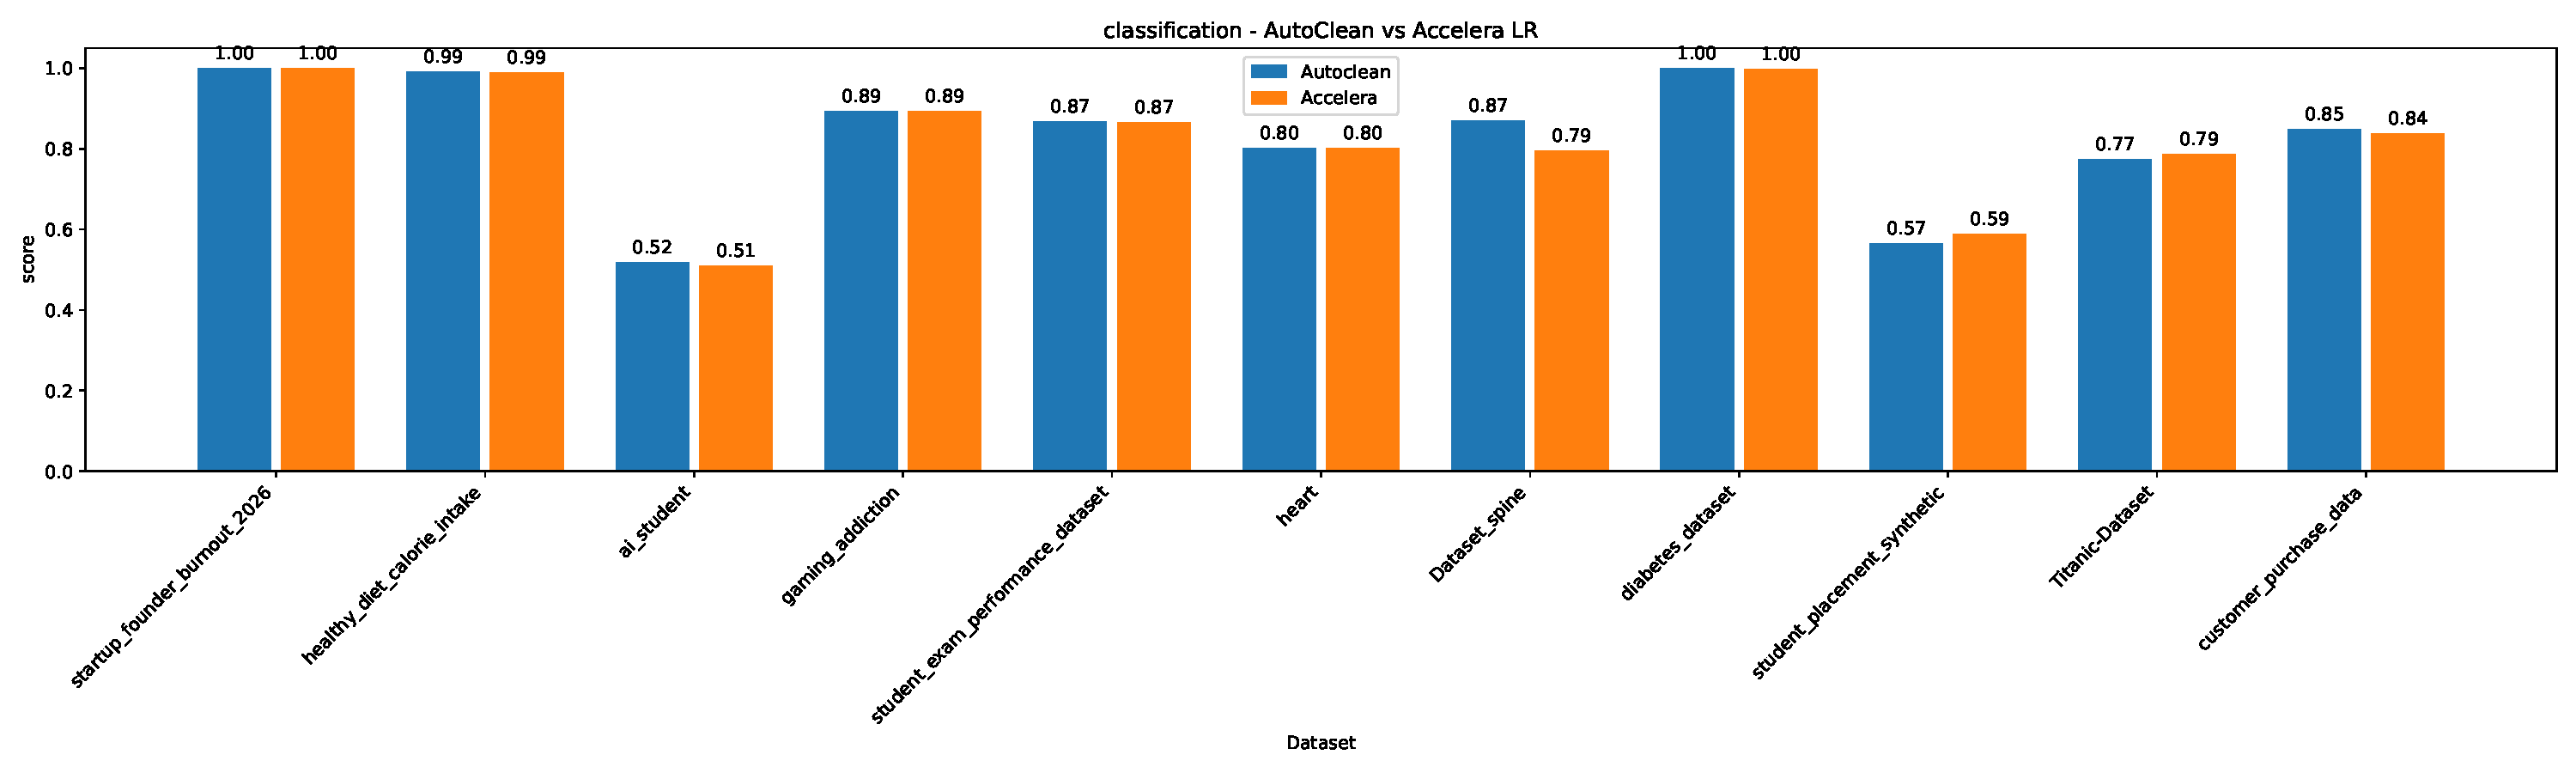
\includegraphics[width=0.48\textwidth]{../imgs/comparison_classification_score_LR.pdf}
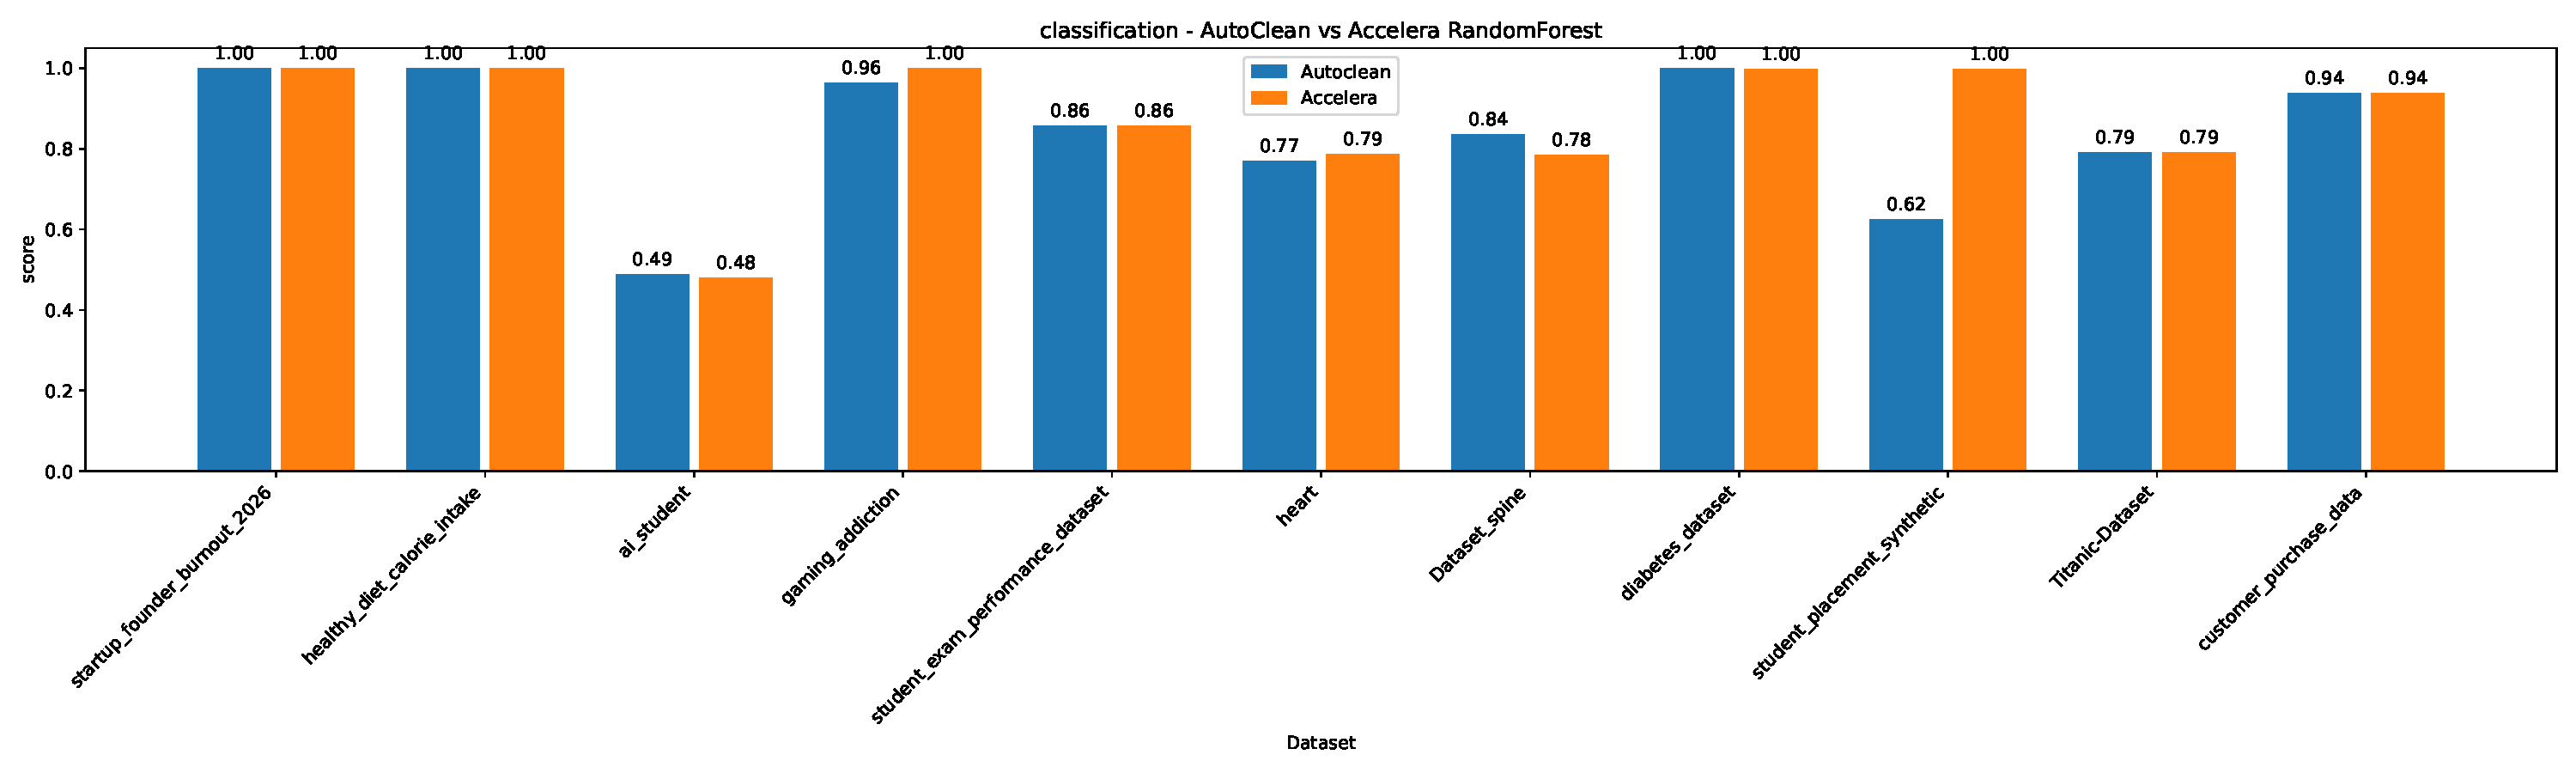
\includegraphics[width=0.48\textwidth]{../imgs/comparison_classification_score_RandomForest.pdf}
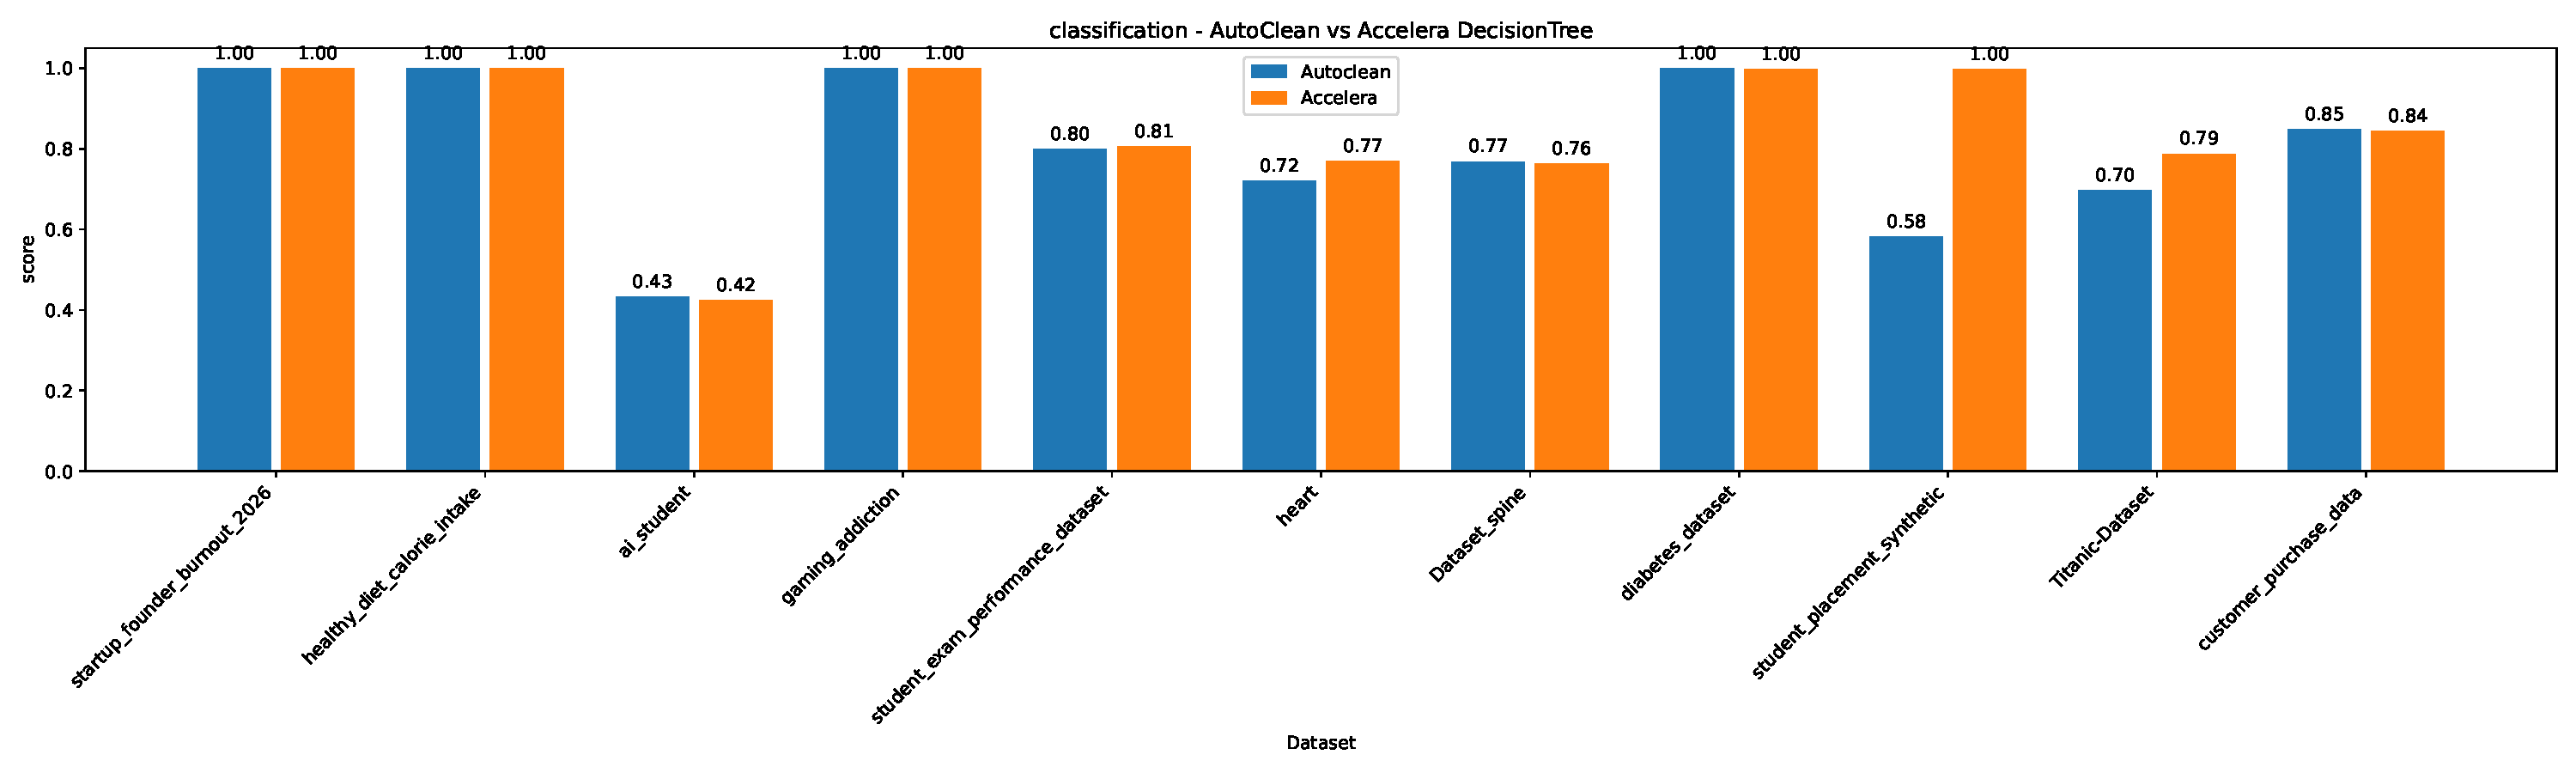
\includegraphics[width=0.48\textwidth]{../imgs/comparison_classification_score_DecisionTree.pdf}
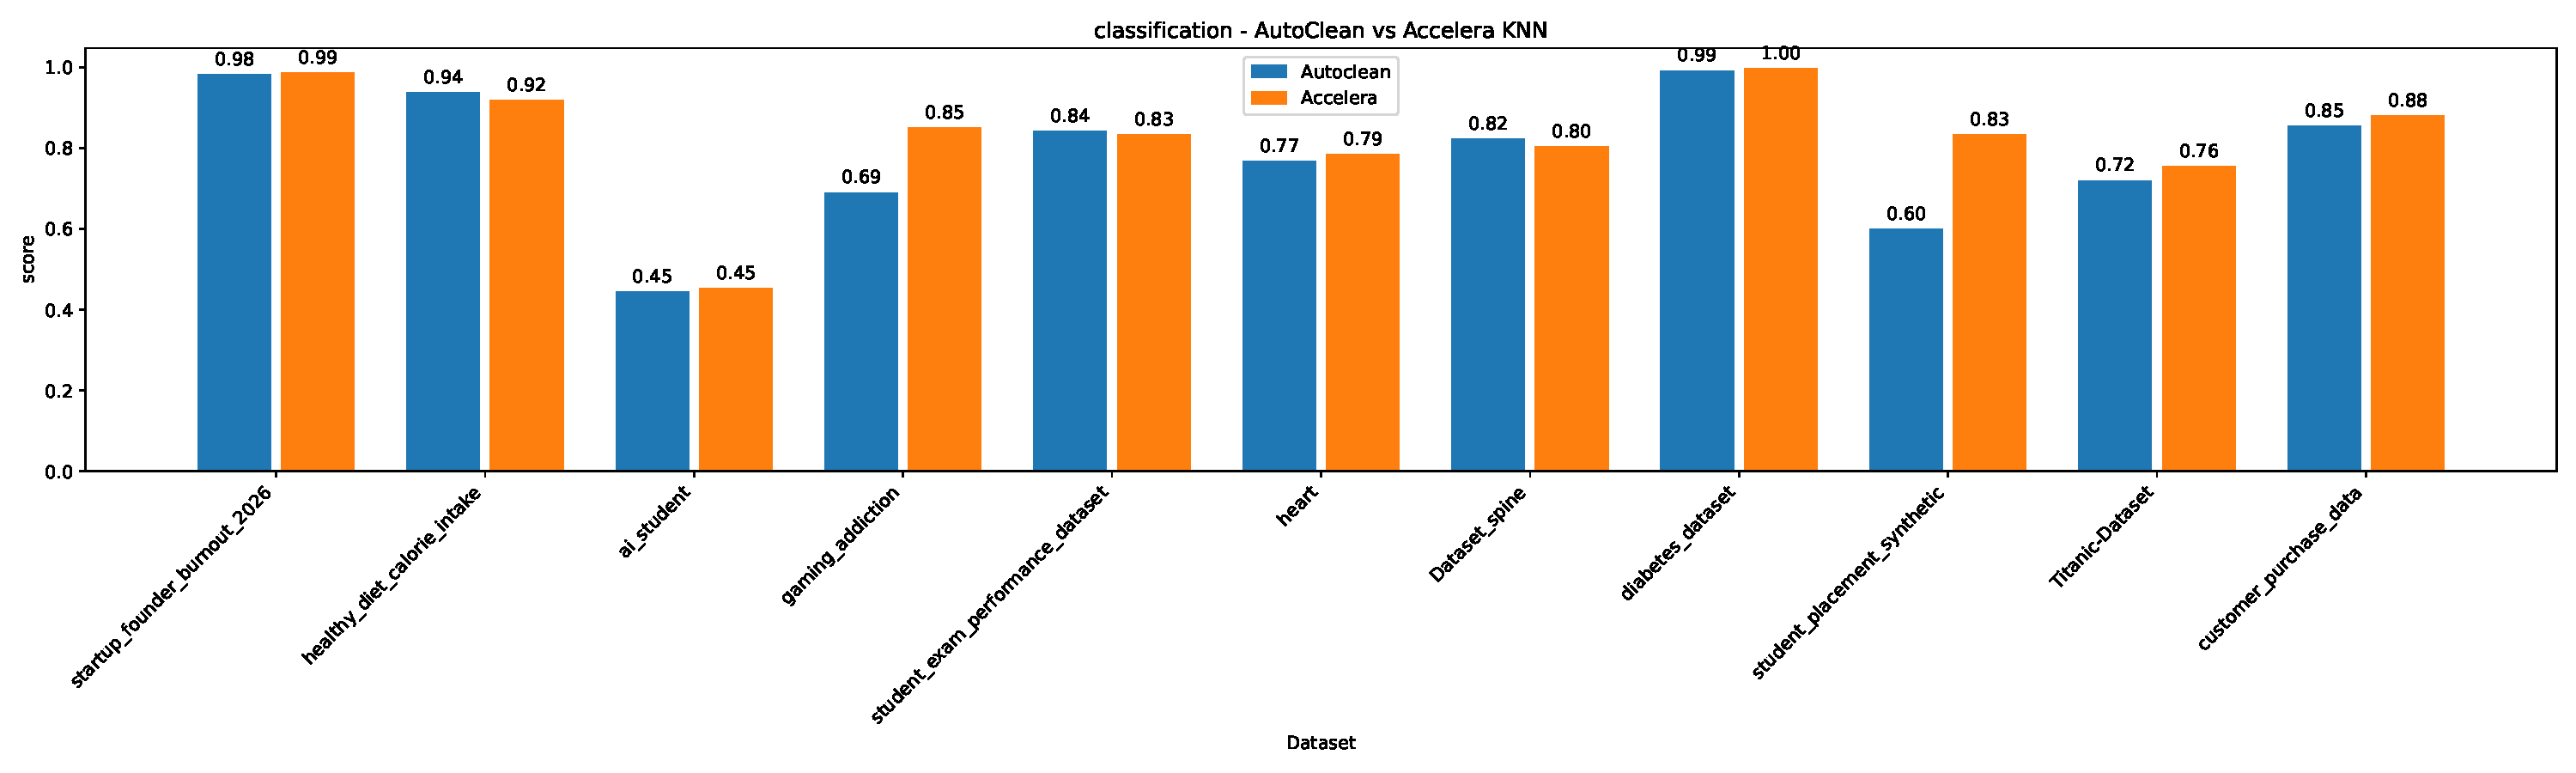
\includegraphics[width=0.48\textwidth]{../imgs/comparison_classification_score_KNN.pdf}
\caption{Classification score comparison graphs for the four tested models}
\label{fig:classification-comparison-graphs}
\end{figure}

\begin{figure}[H]
\centering
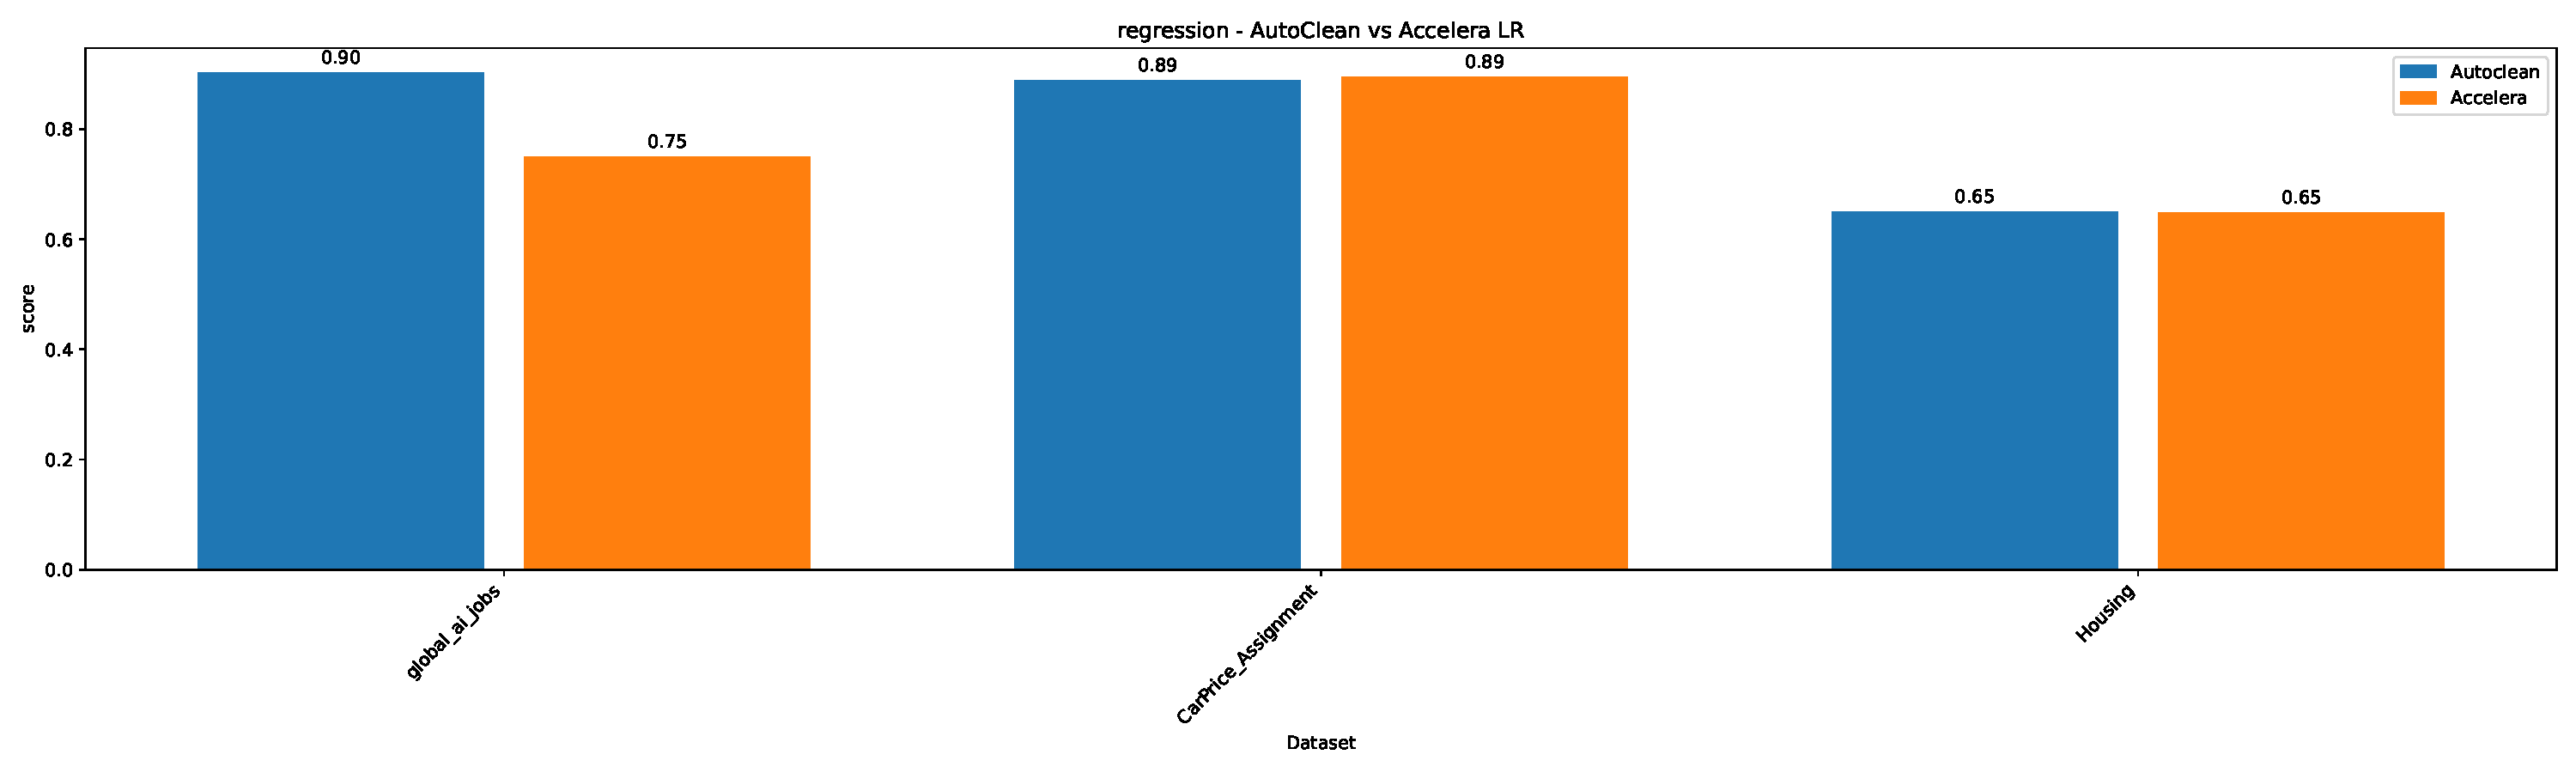
\includegraphics[width=0.48\textwidth]{../imgs/comparison_regression_score_LR.pdf}
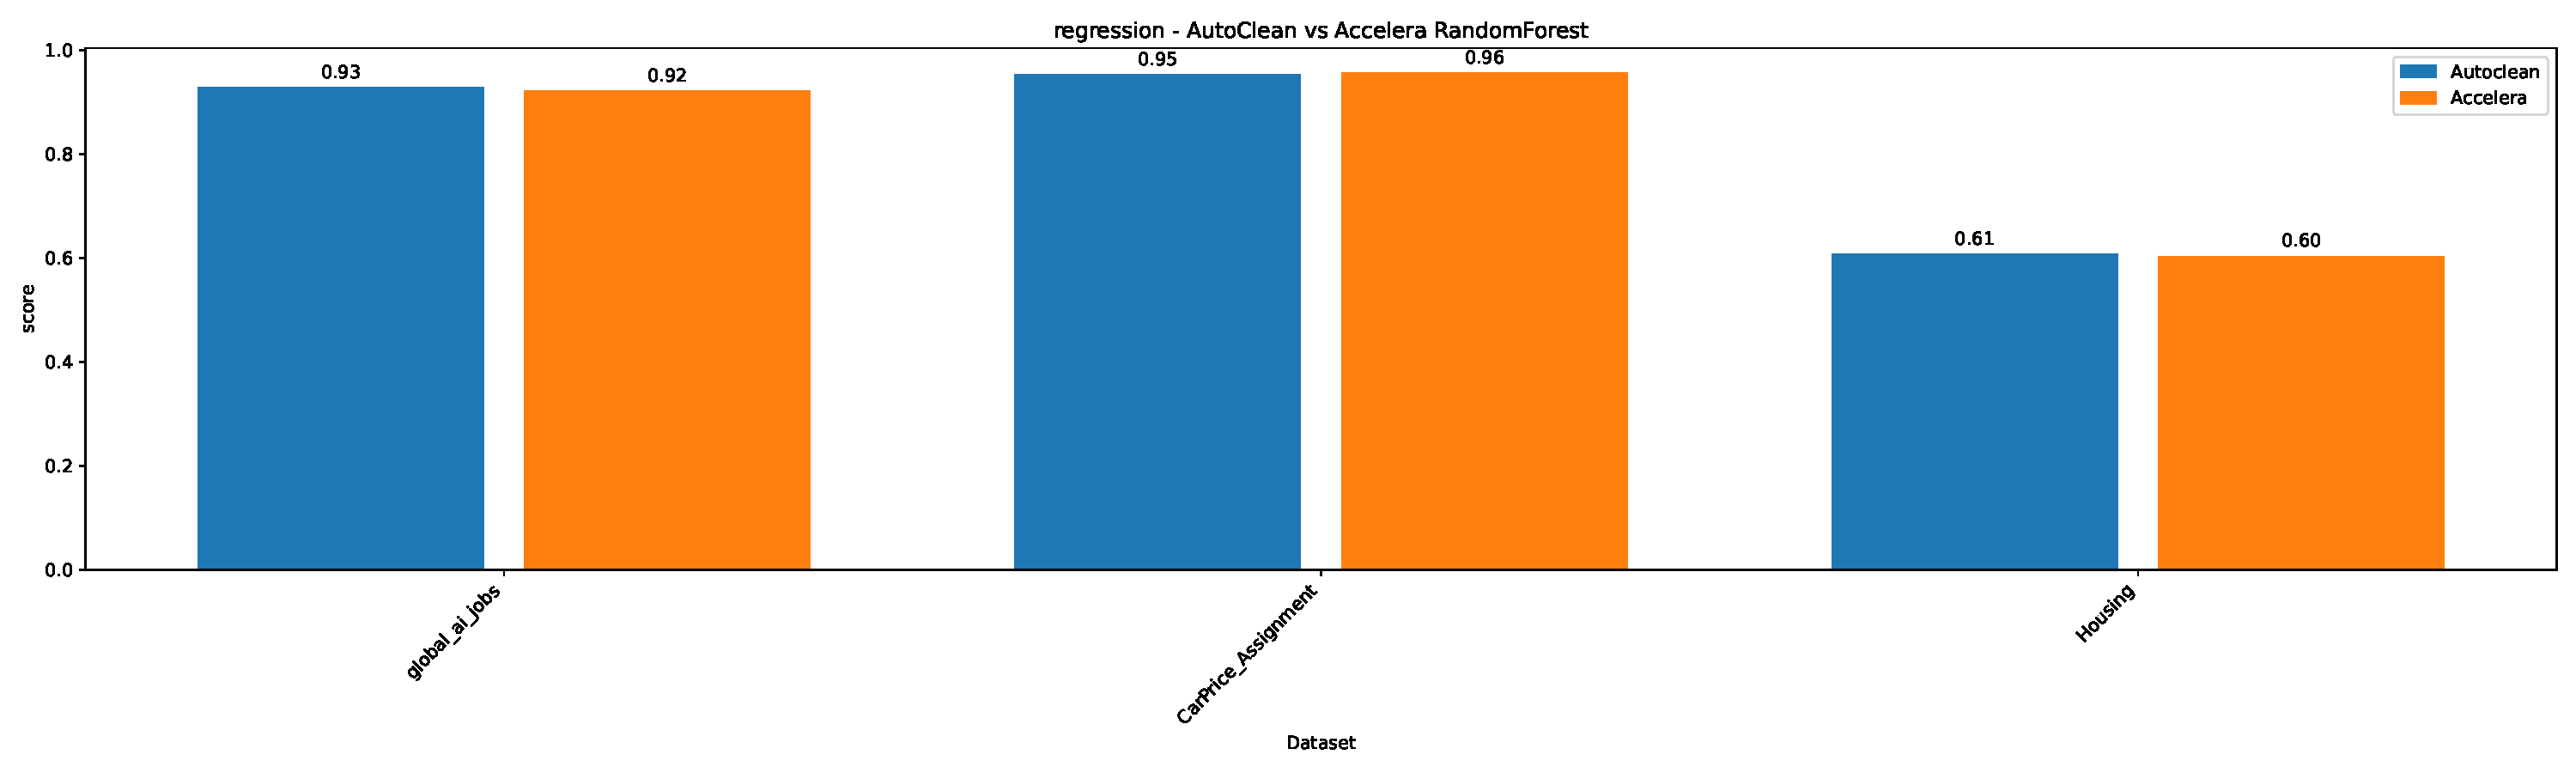
\includegraphics[width=0.48\textwidth]{../imgs/comparison_regression_score_RandomForest.pdf}
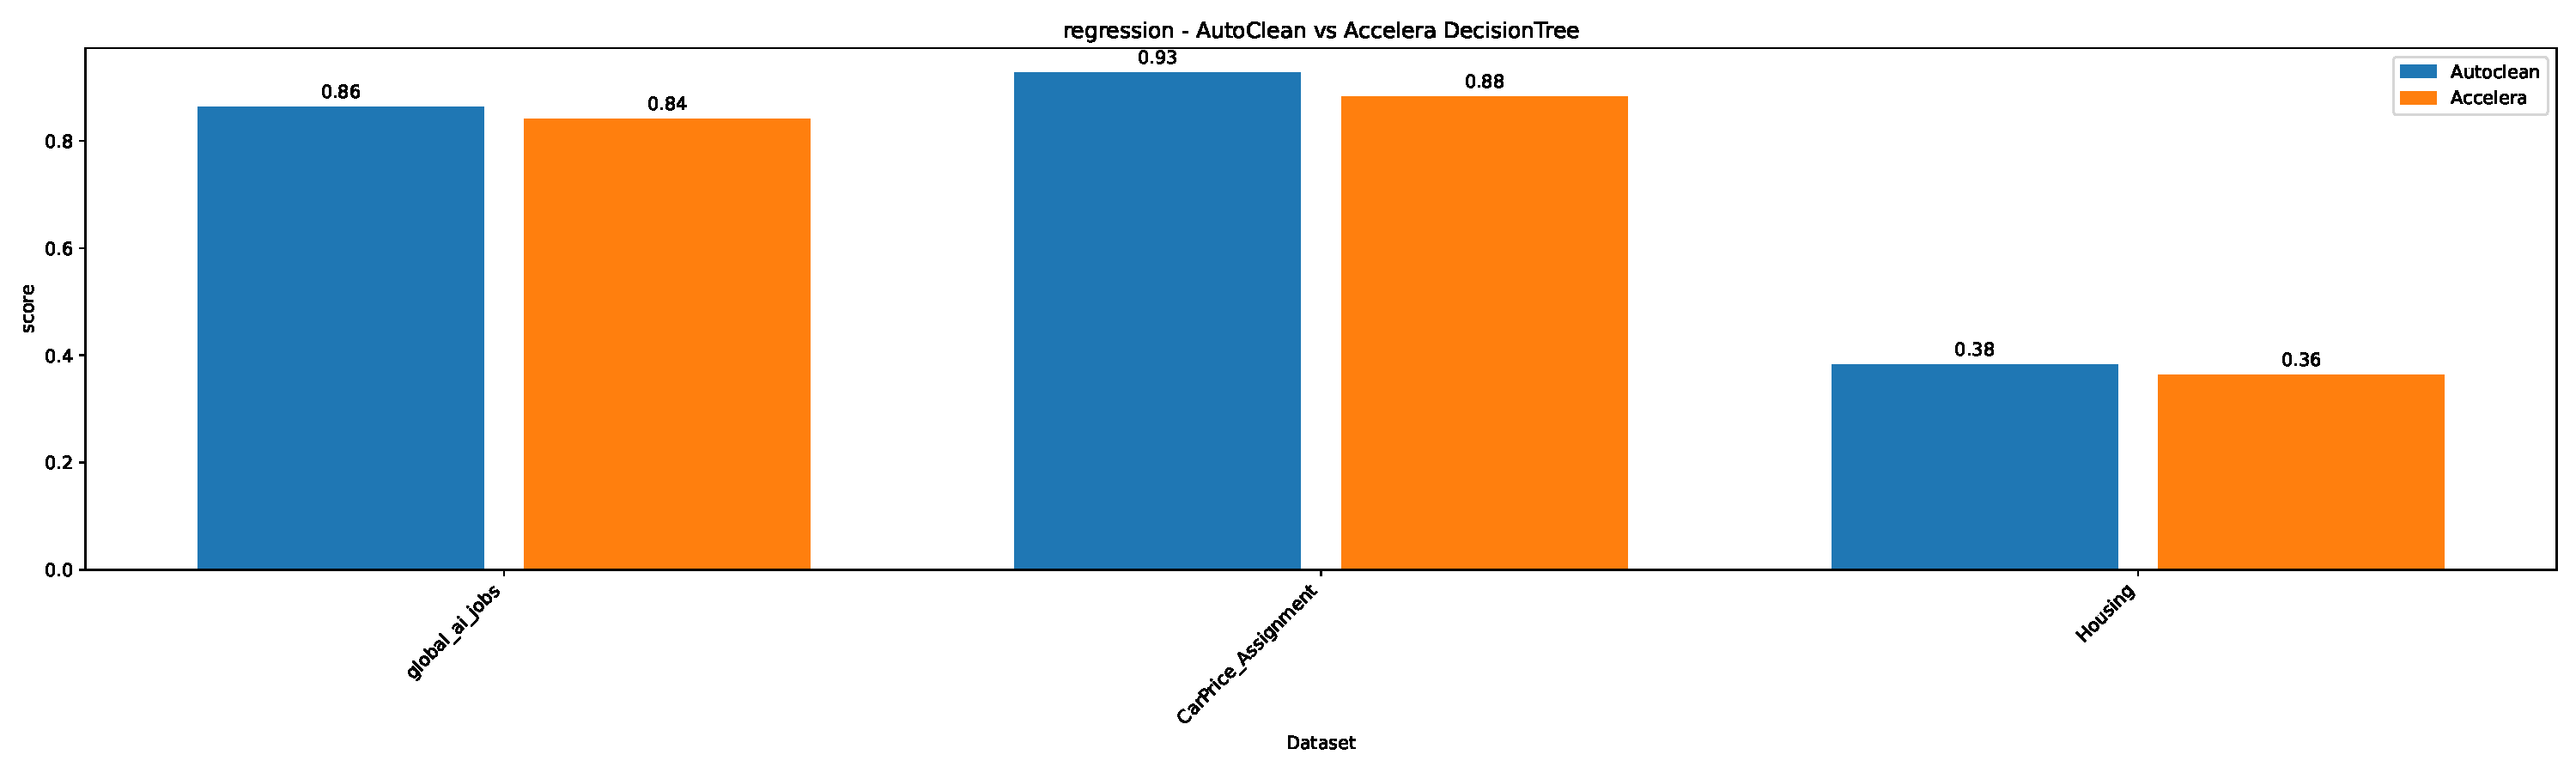
\includegraphics[width=0.48\textwidth]{../imgs/comparison_regression_score_DecisionTree.pdf}
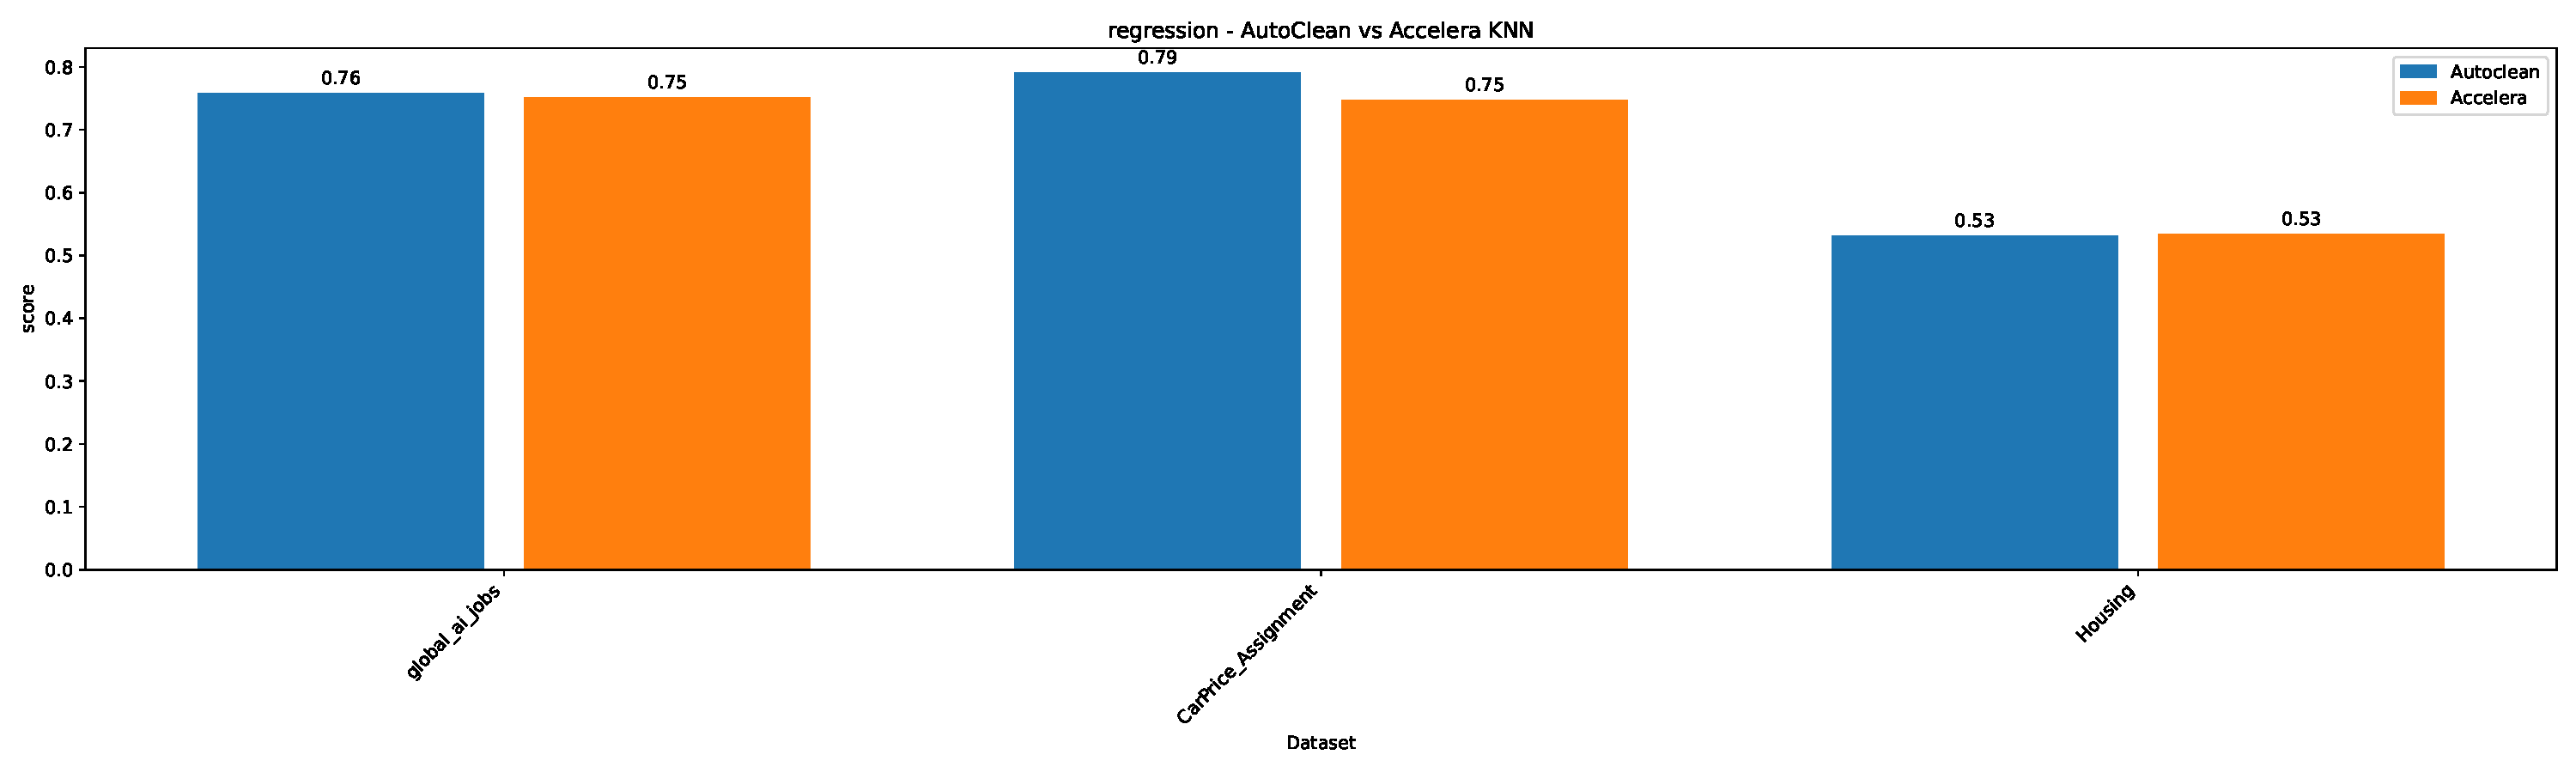
\includegraphics[width=0.48\textwidth]{../imgs/comparison_regression_score_KNN.pdf}
\caption{Regression score comparison graphs for the four tested models}
\label{fig:regression-comparison-graphs}
\end{figure}

From these results, Accelera preprocessing gives very close results to
AutoCleanML in many datasets. In some cases, such as
\texttt{student\_placement\_synthetic}, Accelera gives much higher scores with
tree-based models. In other cases, AutoCleanML is slightly better, especially
in some regression results. This means the Accelera preprocessing output is
valid and competitive, but the best tool can still depend on the dataset and
the model used after preprocessing.

\section{Reporting Module Testing}

The graph report is exercised through examples that build branch-based
workflows, serialize the graph to XML, and run \modulepath{GraphReport}. The
expected result is a \modulepath{report.html} file and a graph image showing
the serialized graph structure. The report also checks that metrics are displayed
according to their result type.

\section{Benchmarking Module Testing}

The Benchmarking module was tested manually by submitting different model
results and checking whether the submitted results were saved and displayed in
the leaderboard. The main checked behavior was that the module receives a
submission, stores the dataset name, metric name, and score, and orders the
leaderboard correctly.

\section{Testing Datasets}

\begin{table}[H]
\centering
\caption{Examples of datasets used in Auto Preprocessing testing}
\label{tab:testing-datasets}
\begin{tabular}{p{0.45\textwidth}p{0.20\textwidth}p{0.25\textwidth}}
\toprule
Dataset & Data type & Problem type \\
\midrule
\modulepath{startup_founder_burnout_2026} & Tabular & Classification \\
\modulepath{healthy_diet_calorie_intake} & Tabular & Classification \\
\modulepath{ai_student} & Tabular & Classification \\
\modulepath{Titanic-Dataset} & Tabular & Classification \\
\modulepath{global_ai_jobs} & Tabular & Regression \\
\modulepath{CarPrice_Assignment} & Tabular & Regression \\
\modulepath{Housing} & Tabular & Regression \\
\modulepath{PetImages} & Image & Classification \\
\modulepath{DailyDialog} & Text & Classification \\
\modulepath{TestReviews} & Text & Classification \\
\bottomrule
\end{tabular}
\end{table}

% -----------------------------------------------------------------------------
\chapter{Discussion}
\label{chap:discussion}

\section{Design Advantages}

The main advantage of Auto Preprocessing is consistency. The same fitted
objects used during training are saved and loaded during testing. This reduces
the chance of data leakage and mismatched transformations. Another advantage is
that the module supports more than one data type, so the same project can
prepare tabular, text, and image datasets.

The main advantage of the Reporting module is explainability. The user can see
data summaries, generated visualizations, preprocessing decisions, graph
structure when available, and metric results in one place.

The Benchmarking module helps make comparison fairer because all submissions
are evaluated using the same ground truth and metric configuration.

\section{Current Limitations}

There are also limitations:

\begin{itemize}[leftmargin=*]
  \item the preprocessing rules are fixed heuristics and may not be optimal for
        every dataset;
  \item the tabular preprocessing path assumes ordinary structured data and may
        need extensions for time-series or special domain data;
  \item text preprocessing uses classical TF-IDF, not transformer-based
        language models;
  \item image preprocessing prepares data loaders but does not automatically
        choose the best neural network architecture;
  \item graph report generation depends on graph serialization before
        report execution;
  \item benchmark files are provided through links, so file availability
        depends on external storage; and
  \item the benchmark testing described in the current report is mainly manual.
\end{itemize}

\section{Possible Improvements}

Future improvements can include adaptive preprocessing based on the model type,
better handling of imbalanced datasets, more advanced text preprocessing,
server-side benchmark file storage, stronger automated tests for the
Benchmarking module, and more polished report templates. The graph report can also be
extended to include execution time and memory information for each branch.

% -----------------------------------------------------------------------------
\chapter{Conclusion}
\label{chap:conclusion}

This report documented the Auto Preprocessing module, the Reporting module,
and the Benchmarking module in \systemname{}. The Auto Preprocessing
module automates repeated preparation steps for tabular, text, and image data
and saves artifacts for consistent testing. The Reporting module uses HTML
pages, tables, saved figures, and metric display wrappers to explain outputs.
The Benchmarking module provides a shared
evaluation workflow for comparing prediction submissions using the same metric
and ground truth.

Together, these parts support a more complete data-science workflow. The user
can prepare data, inspect generated reports, and compare final predictions in a
benchmark. The implementation still has limitations, but it gives a clear base
for future development and evaluation.

\begin{thebibliography}{9}

\bibitem{preprocessing_feature_engineering}
Data Preprocessing and Feature Engineering for Data Mining: Techniques, Tools,
and Best Practices.
\newblock Available at:
\url{https://www.proquest.com/openview/17dfa731b6147c8939e3c5cc784897ce/1?pq-origsite=gscholar&cbl=5046920}

\end{thebibliography}

\end{document}
